\documentclass{beamer}
\usepackage[brazilian]{babel}
\usepackage[utf8]{inputenc}
\usepackage[T1]{fontenc}
\usepackage{listings}

\mode<presentation> {

 \usetheme{Frankfurt}
 \setbeamertemplate{footline} % To remove the footer line in all slides uncomment this line
 
 \setbeamertemplate{footline}[page number] % To replace the footer line in all slides with a simple slide count uncomment this line

 %\setbeamertemplate{navigation symbols}{} % To remove the navigation symbols from the bottom of all slides uncomment this line
}

\usepackage{graphicx} % Allows including images
\usepackage{booktabs} % Allows the use of \toprule, \midrule and \bottomrule in tables

%----------------------------------------------------------------------------------------
% TITLE PAGE
%----------------------------------------------------------------------------------------

\title[EP1 - MAC0422]{EP1 - MAC0422 - 2015 \\
                      ep1sh e simproc} % The short title appears at the bottom of every slide, the full title is only on the title page
\author{Renato Lui Geh e Ricardo Fonseca}
\date{}
\begin{document}

\begin{frame}
  \titlepage % Print the title page as the first slide
\end{frame}


%----------------------------------------------------------------------------------------
% PRESENTATION SLIDES
%----------------------------------------------------------------------------------------

%------------------------------------------------
\section{ep1sh} % Sections can be created in order to organize your presentation into discrete blocks, all sections and subsections are automatically printed in the table of contents as an overview of the talk
%------------------------------------------------

\begin{frame}
  \frametitle{Shell}
  No shell ep1sh, além das diversas funções para utilidades, como \texttt{extract\_args} e \texttt{cmd\_exists}, as duas funções mais importantes são \texttt{run\_cmd} e \texttt{run\_ext\_cmd}, que cuidam
  da execução dos comandos.
\end{frame}

\begin{frame}
  \frametitle{\texttt{run\_cmd}}
  \texttt{run\_cmd} roda os comandos embutidos (\texttt{cd}, \texttt{pwd} e \texttt{exit}), este último adicionado para facilitar os testes durante a produção do EP. Nessa função foi feita manualmente apenas \texttt{cd}, já que em \texttt{pwd} podíamos apenas chamar
  \texttt{getcwd} e em seguida imprimirmos na saída padrão, e em \texttt{exit} podemos chamar apenas \texttt{exit(EXIT\_SUCCESS)}. Foram implementados os símbolos especiais \texttt{..}, \texttt{\~} e \texttt{\textbackslash} em
  \texttt{cd}.
\end{frame}

\begin{frame}
  \frametitle{\texttt{run\_ext\_cmd}}
  \texttt{run\_ext\_cmd} roda os comandos \texttt{\textbackslash bin\textbackslash ls -1} e qualquer executável que esteja em \texttt{path}. Para isso cria-se um novo processo com \texttt{fork} e em seguida usa-se o \texttt{execve},
  fazendo o processo pai esperar o processo filho com \texttt{waitpid}.
\end{frame}

%------------------------------------------------

\begin{frame}
  \frametitle{Funções auxiliares}
  Para certas tarefas de manipulação de strings e para saber se existe um comando que foi lido foram feitas duas funções: \texttt{cmd\_exists} e \texttt{extract\_args}. 
\end{frame}

%------------------------------------------------

\begin{frame}
  \frametitle{\texttt{cmd\_exists}}
  Verifica se o comando que o usuário deseja executar é um comando embutido no shell (\texttt{cd}, \texttt{pwd} ou \texttt{exit}). Se for, roda-se \texttt{run\_cmd}, senão precisamos rodar \texttt{run\_ext\_cmd}.
\end{frame}

%------------------------------------------------

\begin{frame}
  \frametitle{\texttt{extract\_args}}
  Separa a linha lida da entrada em tokens separados por espaço. Cada token é então posta em uma posição na tabela de argumentos \texttt{args\_table}. Considera-se o argumento na posição zero como sendo o próprio comando. \\~\\
  
  \textbf{Importante:} a linha lida é então inutilizada, já que usa \texttt{strtok}. Em \texttt{main}, a cada iteração liberamos a memória alocada na variável da linha lida.
\end{frame}
%------------------------------------------------

\begin{frame}
    \frametitle{history}
    Por último utilizamos as bibliotecas readline e GNU history, as quais auxiliam para que nosso shell se comporte como o prompt do linux (as setas direcionais auxiliam na edição do texto)

\end{frame}

%------------------------------------------------
\section{simproc}
%------------------------------------------------

\begin{frame}
  \frametitle{Simulador de processos}
  Para facilitar o trabalho da implementação do nosso Simulador de Processos, criamos dois arquivos: \texttt{utils.c} e \texttt{utils.h}. Nesses arquivos foram criados filas, filas de prioridade e uma estrutura para o processo. \\~\\

  Filas foram implementadas num vetor de forma cíclica para melhorar a complexidade. Filas de prioridade foram implementadas como heaps. Chamamos de \texttt{thread\_clock} o tempo de execução do escalonador.
\end{frame}

%------------------------------------------------

\begin{frame}
  \frametitle{Escalonadores}
  Para ser mais fácil de se escolher qual escalonador usar, criamos a variável \texttt{manager}, que é um ponteiro para função. Os argumentos de linha de comando são lidos e a função é atribuída a \texttt{manager} em seguida. \\~\\

  Além disso alguns escalonadores utilizam filas de prioridade que outros não precisam. Por isso algumas filas nunca são utilizadas se usarmos certo escalonador.
\end{frame}

%------------------------------------------------

\begin{frame}
  \frametitle{Filas}
  Em todos os escalonadores implementados foram usadas as filas \texttt{p\_queue} e \texttt{trace\_procs}. \\~\\
  
  \texttt{p\_queue}: guarda todos os processos que já foram rodados ou que estão rodando ainda. \\~\\

  \texttt{trace\_procs}: guarda todas que ainda não foram rodadas.
\end{frame}

%----------------------------------------------------------------------------------------

\begin{frame}
  \frametitle{First-Come First-Serve (FCFS)}
  Este escalonador usa apenas filas. Quando o \texttt{thread\_clock} chega no instante \texttt{t0} de um processo, se há alguma CPU não utilizada, o processo é atribuído àquela CPU. \\~\\

  O processo permanece na CPU até terminar.
\end{frame}

%----------------------------------------------------------------------------------------

\begin{frame}
  \frametitle{Shortest Job First (SJF)}
  Este escalonador usa uma fila de prioridade com critério de comparação igual a relação de grandeza entre os \texttt{dt}s de cada processo concorrente. \\~\\

  Se não há CPU disponível, o processo entra na fila de prioridade e espera ter uma CPU livre.
\end{frame}

%----------------------------------------------------------------------------------------

\begin{frame}
  \frametitle{Shortest Remaining Time Next (SRTN)}
  Este escalonador é similar ao SJF, com a única diferença que a fila de prioridade tem critério de comparação entre as grandezas dos \texttt{thread\_clock - deadline} de cada processo. \\~\\

  Se não há CPU disponível, o processo entra na fila de prioridade e espera ter CPU livre.
\end{frame}

\begin{frame}
  \frametitle{Round-Robin (RR)}
  Este escalonador disponibiliza um quantum de tempo para cada processo em cada CPU trabalhando. No \texttt{simproc} usamos um quantum \texttt{SCHED\_QUANTUM=0.050} segundos. \\~\\

  Usou-se \texttt{pthread\_cond\_t} e \texttt{pthread\_mutex\_t} para mandar sinais para suspender ou resumir o thread.
\end{frame}

\section{comparação}

\begin{frame}
  \frametitle{Comparações}
  Veremos algumas comparações entre os diferentes escalonadores.
\end{frame}

\begin{frame}
\begin{figure}[h]
  \centering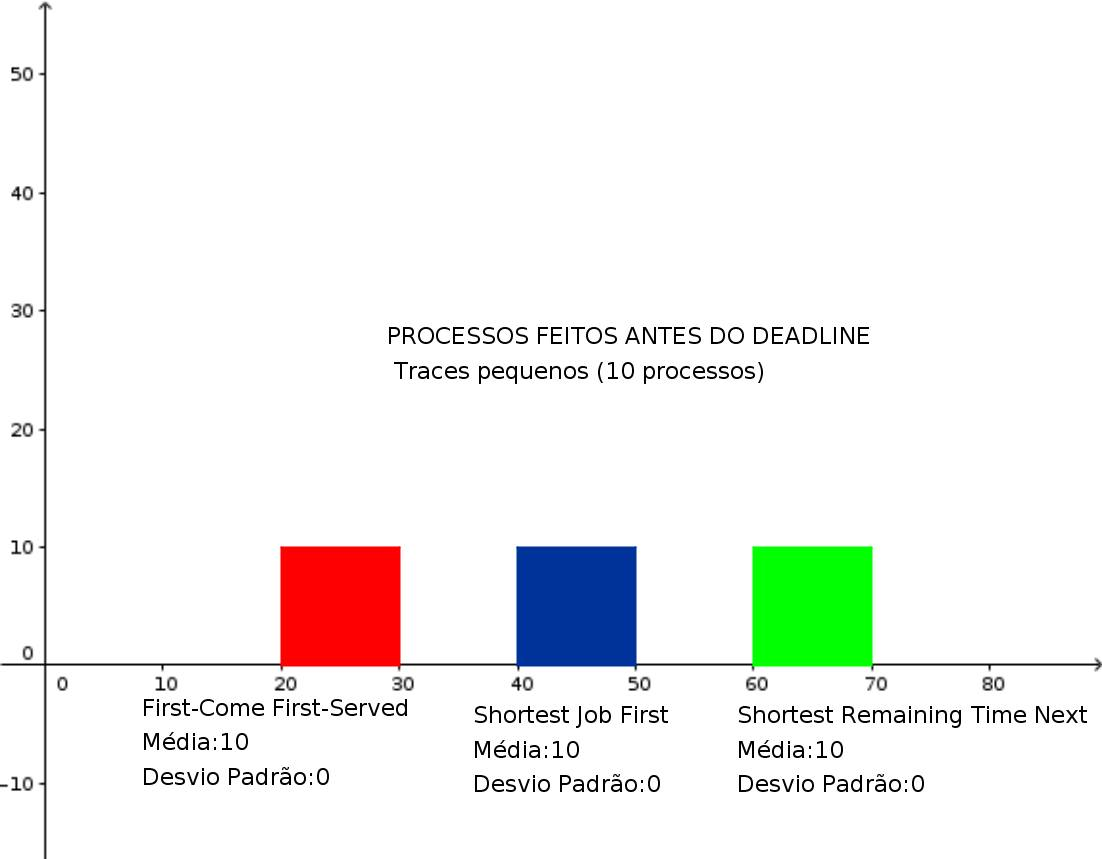
\includegraphics[scale=0.25]{table1.jpg}
\end{figure}
\end{frame}

\begin{frame}
\begin{figure}[h]
  \centering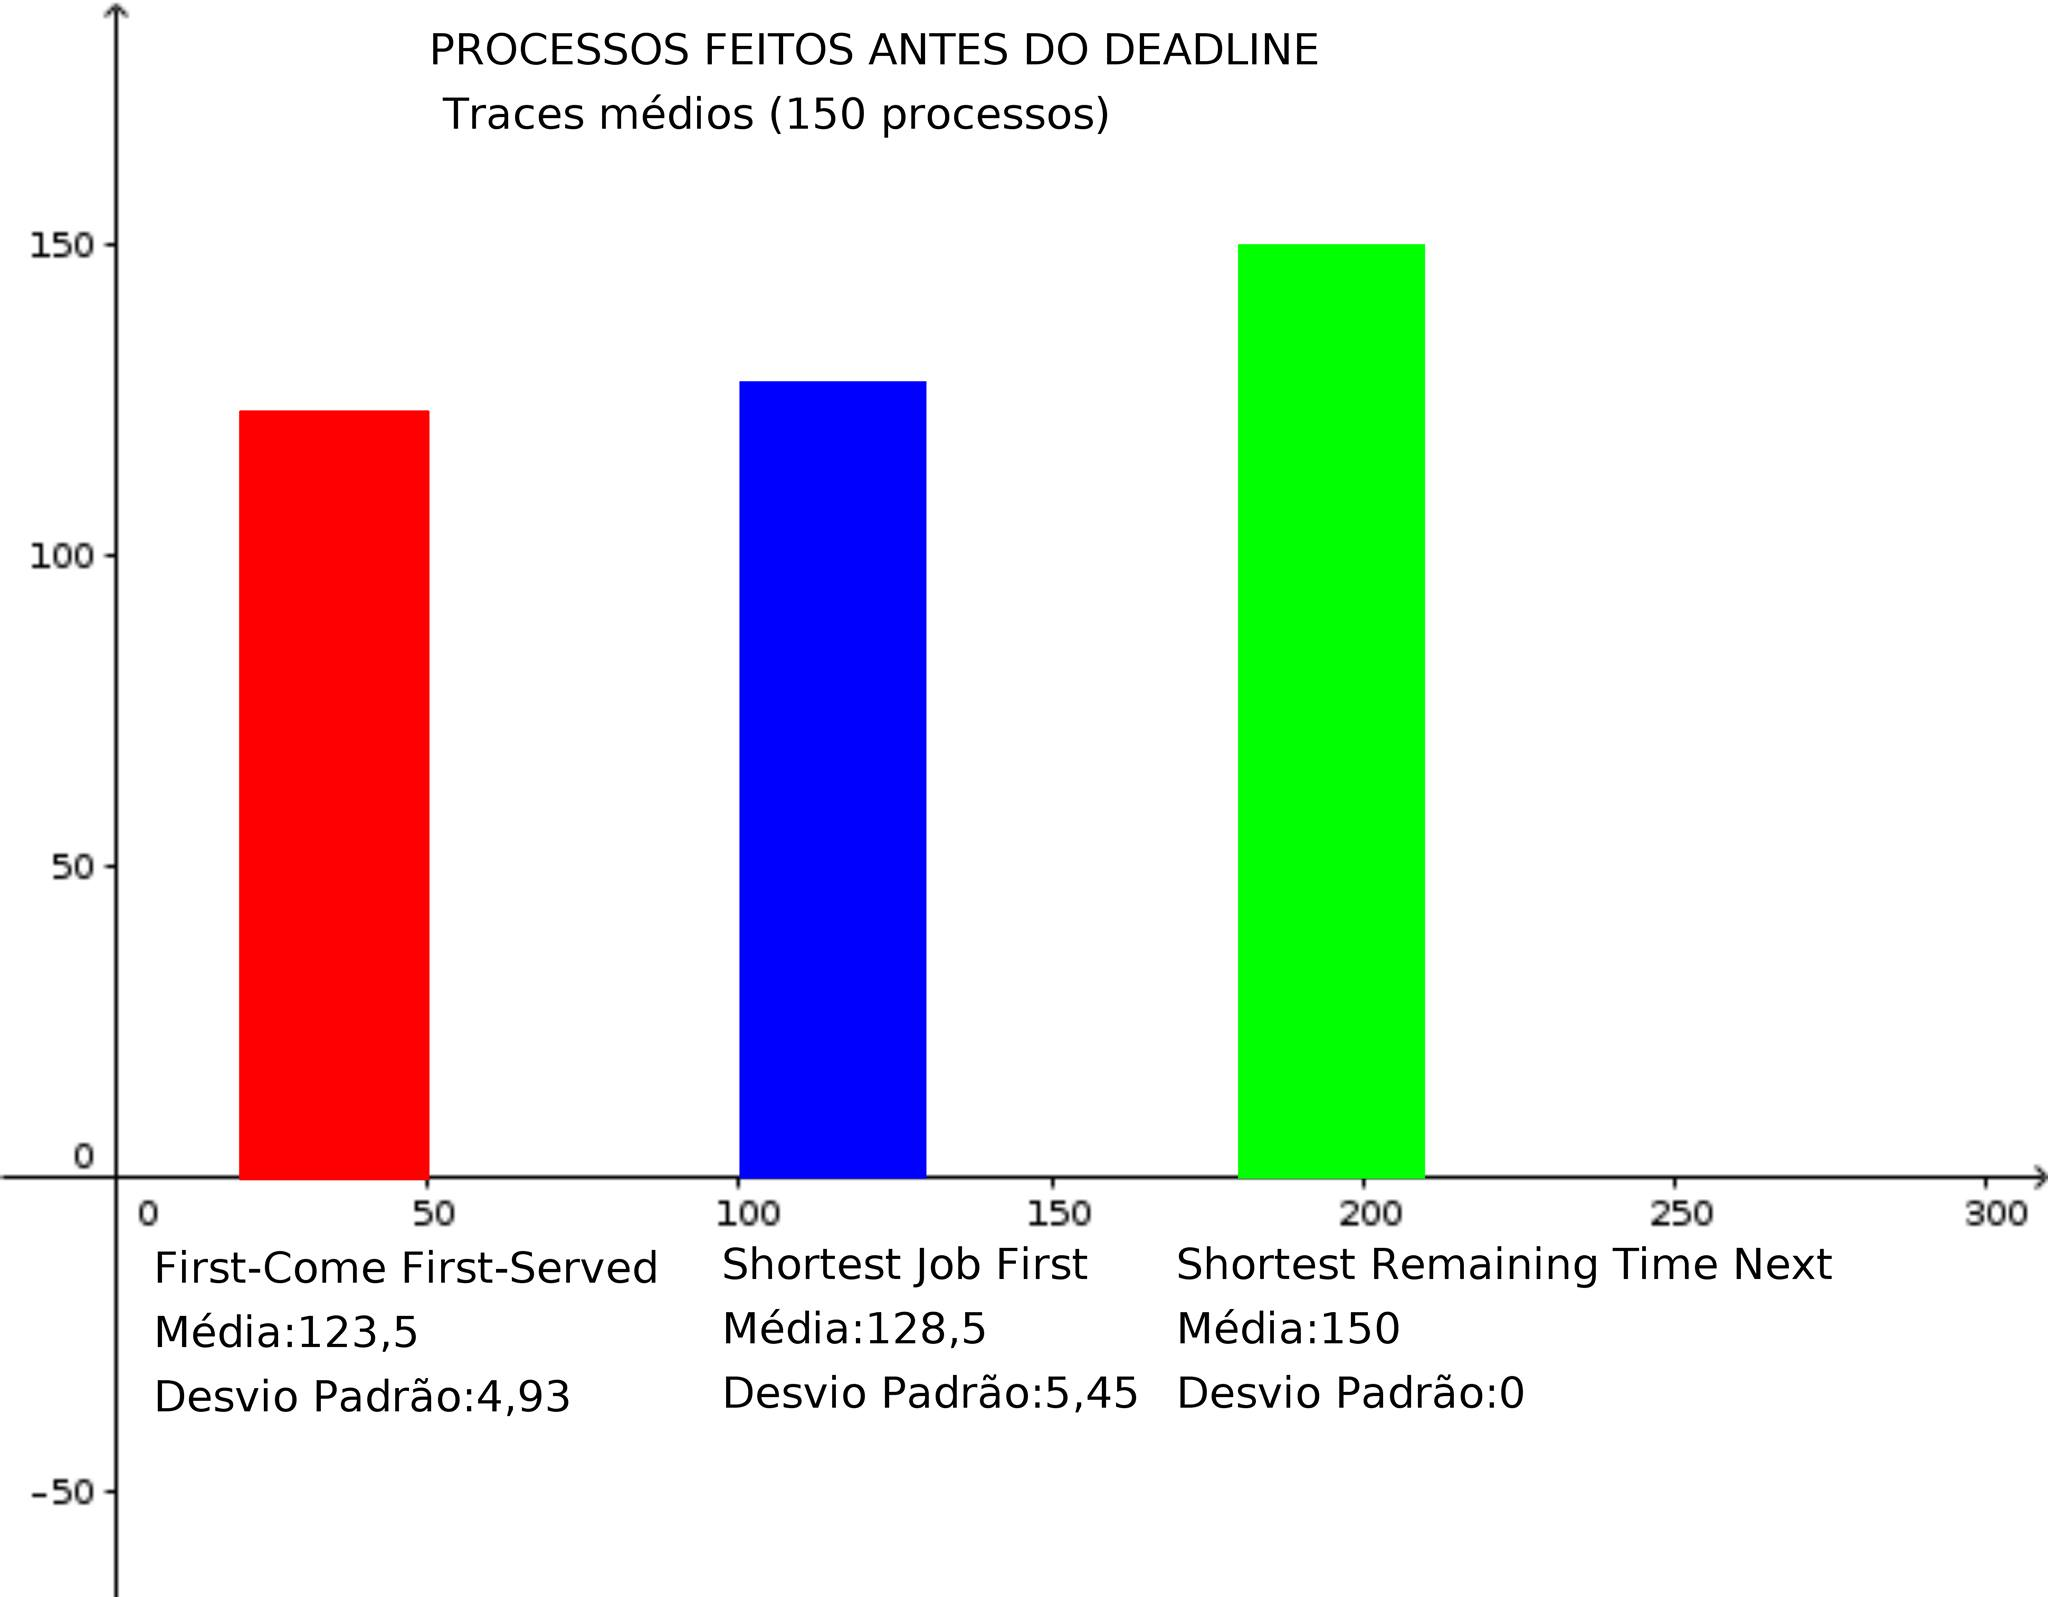
\includegraphics[scale=0.15]{table2.jpg}
\end{figure}
\end{frame}

\begin{frame}
\begin{figure}[h]
  \centering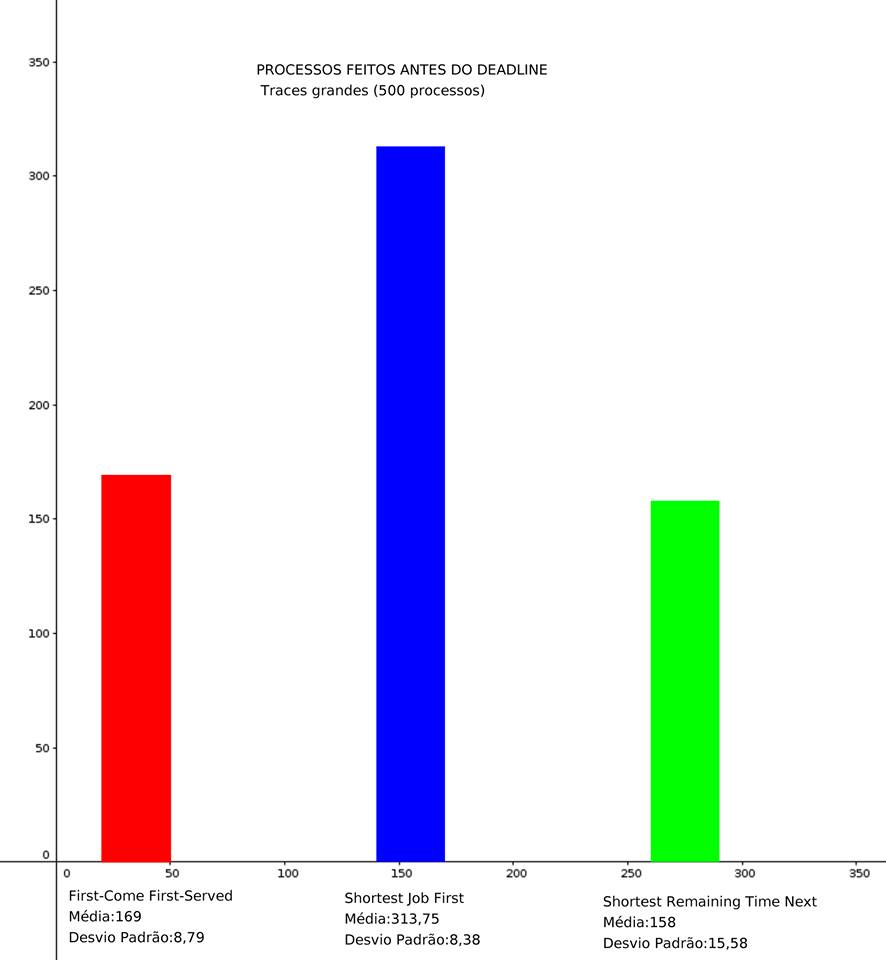
\includegraphics[scale=0.25]{table3.jpg}
\end{figure}
\end{frame}

\end{document}
